\documentclass[conference]{IEEEtran}
\IEEEoverridecommandlockouts
% The preceding line is only needed to identify funding in the first footnote. If that is unneeded, please comment it out.
\usepackage{cite}
\usepackage{amsmath,amssymb,amsfonts}
\usepackage{algorithmic}
\usepackage{graphicx}
\usepackage{textcomp}
\usepackage{xcolor}
\def\BibTeX{{\rm B\kern-.05em{\sc i\kern-.025em b}\kern-.08em
		T\kern-.1667em\lower.7ex\hbox{E}\kern-.125emX}}
\begin{document}
	
\title{Enhancing Reasoning Skills in Small Persian Medical Language Models Can Outperform Large-Scale Data Training}
	
\author{\IEEEauthorblockN{1\textsuperscript{st} Mehrdad Ghassabi}
		\IEEEauthorblockA{\textit{Faculty of Computer Engineering} \\
			\textit{University of Isfahan}\\
			Isfahan, Iran \\
			m.ghassabi@eng.ui.ac.ir}
		\and
		\IEEEauthorblockN{2\textsuperscript{nd} Sadra Hakim}
		\IEEEauthorblockA{\textit{School of Computer Science} \\
			\textit{University of Windsor}\\
			Windsor, Canada \\
			hakim6@uwindsor.ca}
		\and
		\IEEEauthorblockN{3\textsuperscript{rd} Hamidreza Baradaran Kashani}
		\IEEEauthorblockA{\textit{Faculty of Computer Engineering} \\
			\textit{University of Isfahan}\\
			Isfahan, Iran \\
			hrb.kashani@eng.ui.ac.ir }
		\and
		\IEEEauthorblockN{4\textsuperscript{th} Pedram Rostami}
		\IEEEauthorblockA{\textit{School of Electrical and Computer Engineering} \\
			\textit{University of Tehran}\\
			Tehran, Iran \\
			pedram.rostami@ut.ac.ir}
	}
	
	\maketitle
	
	\begin{abstract}
Enhancing reasoning capabilities in small language models is critical for specialized applications such as medical question answering, particularly in underrepresented languages like Persian. In this study, we employ Reinforcement Learning with AI Feedback (RLAIF) and Direct preference optimization (DPO) to improve the reasoning skills of a general-purpose Persian language model. To achieve this, we translated a multiple-choice medical question-answering dataset into Persian and used RLAIF to generate rejected-preferred answer pairs, which are essential for DPO training. By prompting both teacher and student models to produce Chain-of-Thought (CoT) reasoning responses, we compiled a dataset containing correct and incorrect reasoning trajectories. This dataset, comprising 2 million tokens in preferred answers and 2.5 million tokens in rejected ones, was used to train a baseline model, significantly enhancing its medical reasoning capabilities in Persian. Remarkably, the resulting model outperformed its predecessor, gaokerena-V, which was trained on approximately 57 million tokens, despite leveraging a much smaller dataset. These results highlight the efficiency and effectiveness of reasoning-focused training approaches in developing domain-specific language models with limited data availability.
	\end{abstract}
	
	\begin{IEEEkeywords}
		system2 deep learning,small language model,medical language models, RLAIF, direct policy optimization
	\end{IEEEkeywords}
	
	\section{Introduction}

Transformer-based language models
\cite{b1} 
excel at fast, intuitive tasks—such as pattern matching, retrieval, and surface-level text generation—mirroring Kahneman’s concept of “fast thinking”
\cite{b2}.  
However, they struggle with deliberate, multi-step reasoning tasks that require “slow thinking,” particularly in specialized domains such as medicine, where diagnostic accuracy depends on logical inference, evidence evaluation, and error correction.  
This limitation is even more severe in low-resource languages such as Persian, where both high-quality data and compute are scarce.

In 2019, Yoshua Bengio warned that deep learning systems lack true reasoning capacity and called for architectures that support out-of-distribution generalization
\cite{b3}.  
While the transformer architecture was revolutionary, its success has largely come from scaling: larger models and larger datasets yield better performance.  
Yet, despite current large language models having trillions of parameters and being trained on tens of trillions of tokens, they still make surprisingly simple reasoning errors.  
They may even produce inconsistent answers when asked the same question directly or via chain-of-thought (CoT) prompting
\cite{b4}.  
This deficiency becomes even more pronounced in small medical Persian language models, which have far fewer parameters and much less training data.

Recent advances have attempted to improve the reasoning ability of language models—enhancing their performance on “slow thinking” tasks—but these methods often rely on large, well-curated datasets available only for high-resource languages such as English or Chinese.  
In contrast, Persian lacks sufficient high-quality medical datasets.  
To address this gap, we propose a new framework to improve the reasoning capabilities of Persian medical language models under limited data availability.

In our proposed method, we machine-translated an English multiple-choice medical question answering dataset into Persian and applied reinforcement learning from AI feedback (RLAIF)
\cite{b5} and direct preference optimization (DPO)
\cite{b6} to enhance the reasoning ability of a baseline Persian medical model.  
The resulting model is named gaokerena-R.
\footnote{All of our work is open-source and available at github.com/Mehrdadghassabi/Gaokerena-R}

Our prior work, gaokerena-V
\cite{b7}, fine-tuned a Persian medical language model using approximately 57 million tokens (including a portion of a medical corpus and a dataset) via supervised fine-tuning (SFT).  
Although gaokerena-V demonstrated strong medical knowledge, gaokerena-R outperforms it when given chain-of-thought prompts—despite being trained on less medical data.  
Since both models share the same baseline model, aya-expanse-8b
\cite{b8}, we hypothesize that enhancing reasoning skills is more beneficial than scaling data for small, low-resource medical language models.

In summary, our contributions are as follows:

\begin{enumerate}
  \item An efficient RLAIF+DPO framework that generates high-signal CoT preference pairs using a teacher–student loop.
  \item gaokerena-R
\footnote{Available at huggingface.co/gaokerena/gaokerena-r1.0}
, an 8b-parameter medical model demonstrating that reasoning-focused training outperforms data scaling in low-resource medical NLP.
  \item A machine-translated Persian medical multiple-choice question answering dataset designed for reasoning-focused model training.
\end{enumerate}

	
	\section{Related Work}
To the best of our knowledge, no prior work has focused on developing Persian medical reasoning language models. Existing Persian medical language models, including gaokerena-V, mainly address knowledge representation and general language understanding with limited attention to reasoning.

 L. Pan et al. reviewed several valuable studies on enhancing reasoning capabilities in language models
\cite{b9}.
Accordingly, we focus here on English-language works that offer methodological insights into generating and integrating reasoning data for improving medical language models.
	\subsection{Related Work In Medical Domain}
One of the notable efforts in developing small-scale medical reasoning language models is MedSSS
\cite{b10}.
This framework focuses on fine-graining the intermediate reasoning steps to enhance the reasoning ability of medical models. To accomplish this, the authors applied the Monte Carlo Tree Search (MCTS)
\cite{b11}
algorithm on medical multiple-choice question-answering datasets to synthesize structured reasoning trajectories using a policy model. Based on this approach, they constructed three datasets supporting different stages of training: a dataset for Supervised Fine-Tuning (SFT) of the policy model, a rejected–preferred answer dataset for Direct Preference Optimization (DPO)
\cite{b12}
,and a soft dual-side label dataset for fine-tuning the Process Reward Model (PRM).Finally, the trained Policy Model was used as the primary reasoning policy, while the trained Process Reward Model acted as a decoding guide to refine and evaluate the reasoning process during generation.

Another significant contribution in this field is MedReason
\cite{b13}. 
In this work, the authors leveraged a structured medical knowledge graph to transform conventional question–answer (Q\&A) pairs into detailed medical reasoning trajectories. Each trajectory represented the step-by-step logical pathway connecting a clinical question to its correct answer, grounded in medical knowledge relationships such as symptoms, diagnoses, treatments, and physiological mechanisms. By constructing a reasoning-enriched dataset in this manner, the authors were able to fine-tune a baseline language model on these structured reasoning examples. This approach led to a marked improvement in the model’s ability to perform reasoning-intensive tasks within the medical domain, demonstrating the effectiveness of incorporating knowledge graph–based reasoning supervision into the training process. The findings from MedReason further emphasize the importance of structured reasoning representations as a means of improving the interpretability and analytical depth of medical language models.

Another important advancement in the development of medical reasoning models is HuatuoGPT-o1
\cite{b14}. 
In this work, the authors introduced a verification-guided reasoning framework designed to improve the logical consistency and accuracy of generated reasoning trajectories. Specifically, they employed a verifier model to assess and guide the policy model during reasoning generation, ensuring that each reasoning path adhered closely to factual correctness and medical plausibility. By filtering and refining reasoning trajectories through this verification process, they created a high-quality dataset composed of verified reasoning sequences. The authors then leveraged both supervised fine-tuning and reinforcement learning techniques to train their baseline language model using these verified data. This dual training approach allowed the model to not only imitate correct reasoning behaviors but also internalize reasoning principles through reward-driven optimization. As a result, HuatuoGPT-o1 demonstrated significant improvements in reasoning accuracy and reliability across a variety of medical question-answering and diagnostic tasks, highlighting the potential of verifier-guided learning frameworks in advancing medical reasoning language models.


         \subsection{Related Work In Other Domain}
Perhaps the most influential recent work in the broader field of AI reasoning is DeepSeek-R
\cite{b15}. Building upon the DeepSeek-V3-Base model, the authors introduced a reinforcement learning framework based on Gradient Regularized Policy Optimization (GRPO)
\cite{b16} 
to explicitly enhance the model’s reasoning capabilities. In this setup, the reinforcement learning process was guided by a reward function specifically designed to evaluate and maximize reasoning performance. Through this training paradigm, DeepSeek-R demonstrated remarkable improvements in logical reasoning and problem-solving accuracy across various benchmarks.  
However, the application of reinforcement learning also introduced several side effects. While reasoning performance improved substantially, the model’s readability and linguistic coherence deteriorated, and instances of language mixing became more frequent. To address these issues, the authors incorporated a small amount of cold-start supervised data and adopted a multi-stage training pipeline. This additional fine-tuning phase helped restore natural language fluency and readability while retaining the strong reasoning skills acquired through reinforcement learning. The resulting model, DeepSeek-R, thus represents a critical step forward in reasoning-oriented AI, demonstrating that reinforcement learning can significantly enhance reasoning ability—provided it is balanced with targeted fine-tuning to maintain linguistic quality.

Another notable contribution in the area of reasoning enhancement is Thought Preference Optimization (TPO)
\cite{b17}. 
In this work, the authors proposed a preference-based framework for improving reasoning quality in language models. Given a question, the model first generates multiple candidate reasoning trajectories. These responses are then evaluated by a judge model, which identifies the best and worst samples based on reasoning correctness and coherence. The collected best–worst pairs are subsequently used to train the baseline model through Direct Preference Optimization (DPO), encouraging it to prefer higher-quality reasoning paths. This approach effectively aligns the model’s reasoning process with human-like evaluative feedback, demonstrating that reasoning quality can be substantially improved through structured preference optimization rather than relying solely on scale or supervised data.

Another relevant study was conducted by N. Ho et al.
\cite{b18},
who explored the transfer of reasoning capabilities from large language models to smaller ones. In their approach, a smaller model was fine-tuned using data generated by a larger model that exhibited stronger reasoning performance. The larger model produced reasoning trajectories and question–answer pairs that served as high-quality supervision signals for the smaller model. Through this distillation process, the smaller model effectively learned reasoning strategies and problem-solving patterns from its larger counterpart, achieving competitive reasoning performance with significantly reduced computational cost. This work demonstrates that reasoning ability can be efficiently transferred across models of different scales through targeted fine-tuning on reasoning-oriented synthetic data.
          \section{Proposed Methods}
Two methods has been porposed. the first one, depicted in Figure \ref{fig1}, utilizes a teacher model (we used DeepSeek-R), which is itself a reasoning language model, to correct the student model’s medical reasoning mistakes in its response to the given multiple choice question.
(if the student model chose the correct option we move to the next question in our dataset)
When provided with the correct answer, the teacher generates a detailed chain-of-thought explanation that highlights the reasoning behind the solution. In this setup, the teacher’s output serves as the preferred answer, while the student’s original response is treated as the rejected answer for Direct Policy Optimization (DPO).

The second method, illustrated in Figure \ref{fig2}, employs the teacher model to provide more granular feedback by identifying specific errors in the student model’s answer to a given multiple-choice question. Upon receiving this feedback, the student model is prompted to correct its response precisely from the point where the error occurred.  Through this iterative process, the student gradually refines its reasoning trajectory and converges on the correct answer.  
This constructive feedback allows the student model to develop reasoning independence, as it learns to correct its own mistakes rather than simply mimicking the teacher’s response.In this setup, the final answer generated by the student is considered the preferred response, while its initial attempt serves as the rejected one for DPO.  
Although this second framework is more time-consuming due to the iterative feedback process, it simplifies DPO training, since both the rejected and preferred answers are generated entirely by the student model itself as sequences of its own tokens.

Due to hardware limitations and the time efficiency of Framework 1, we trained the baseline model, aya-expanse-8b, using Framework 1 for 95\% of the data and Framework 2 for the remaining 5\%. This approach allowed us to efficiently train the model using Direct Preference Optimization (DPO). In total, the training involved 11,000 preferred–rejected answer pairs, containing approximately 2 million tokens in the preferred answers and 2.5 million tokens in the rejected ones.
\begin{figure}[h]
    \centering
    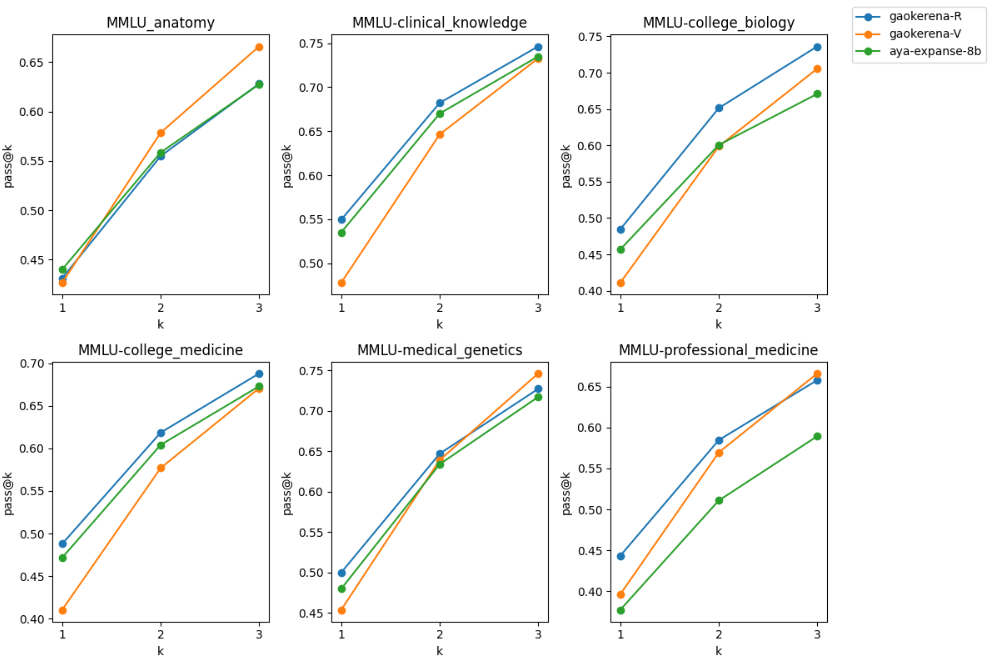
\includegraphics[width=1.0\linewidth]{fig1.png}
    \caption{Method 1 Block Diagram}
    \label{fig1}
\end{figure}

\begin{figure}[h]
    \centering
    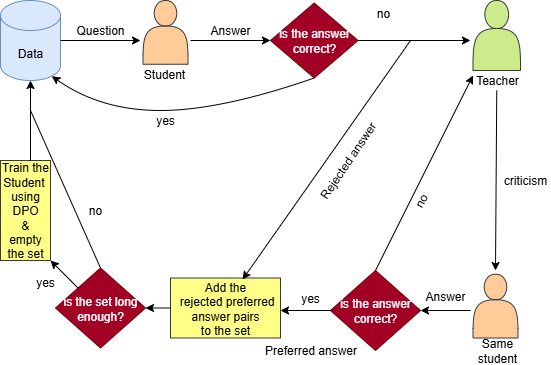
\includegraphics[width=1.0\linewidth]{fig2.png}
    \caption{Method 2 Block Diagram}
    \label{fig2}
\end{figure}


         \section{Data}
We required a Persian medical multiple-choice question answering dataset to implement our proposed method.  
In the absence of such a dataset at the time, we used DeepSeek-V3
\cite{b19}, a cost-effective large language model, to translate a subset of the MedMCQA dataset from English to Persian.  
To maintain topic diversity, the questions were randomly selected from MedMCQA
\cite{b20}.  
To verify the quality of the translations, we prompted
\footnote{Prompts are available at github.com/Mehrdadghassabi/Gaokerena-R/blob/main/dataset/judgement.ipynb}
 two referees—grok-3-mini
\cite{b21} and gpt-4.1-mini
\cite{b22}—to evaluate each translation.  
A translation was considered verified only if both referees assigned it a score of 5 out of 5.  
This process resulted in approximately 18,000 verified Persian medical multiple-choice questions.

         \subsection{PersianMedQA}
Shortly after completing our translation process, a new Persian medical multiple-choice question answering dataset, called PersianMedQA, was introduced
\cite{b23}.  
We randomly selected 1,000 questions from its training set and appended them to our dataset to incorporate additional data from a different source.  
The resulting dataset contained 19,000 Persian medical multiple-choice questions in total.

          \section{Carbon Footprint}
The carbon footprint of our DPO fine-tuning process was estimated based on the hardware configuration and total runtime. The procedure ran for a combined total of 1 hour on an NVIDIA H100 PCIe 80 GB GPU, with approximately 43 GB of VRAM utilized during training. The training loss curve is shown in Figure \ref{fig3}. Assuming an average power consumption of 350 watts per GPU, the total energy usage was approximately 0.35 kWh. Using the average carbon intensity of the Canadian electricity grid, where our server was located (0.086 kilograms of CO2 equivalent per kWh \cite{b24}), this corresponds to an estimated emission of 0.0301 kilograms of CO2 equivalent generated during the fine-tuning process. Compared to our previous model, gaokerena-V, which emitted 2.66 kilograms of CO2, this represents a substantial reduction in environmental impact.\cite{b25}


\begin{figure}[h]
    \centering
    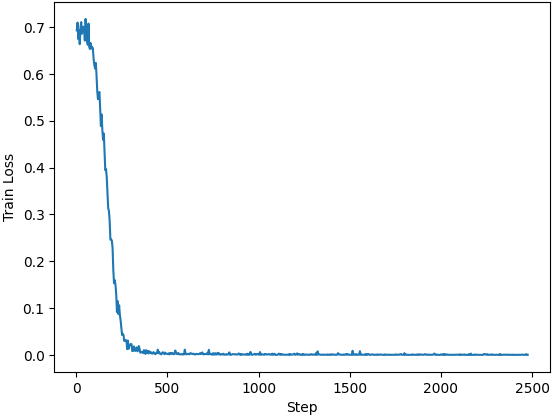
\includegraphics[width=0.8\linewidth]{fig3.png}
    \caption{Training loss curve}
    \label{fig3}
\end{figure}
          \section{Results}
In this section, we compare the newly developed gaokerena-R model with its predecessor, gaokerena-V. While gaokerena-V was trained on a large medical corpus and demonstrates strong factual knowledge and retrieval capabilities, gaokerena-R was specifically designed to enhance medical reasoning. Owing to its reasoning-focused training pipeline, gaokerena-R was trained on a substantially smaller dataset, resulting in slightly reduced coverage of general medical knowledge. However, this trade-off enabled it to develop deeper reasoning competence, allowing it to perform better on tasks requiring multi-step inference and logical consistency.  

In the final evaluation, we compared the performance of gaokerena-V under direct (straight) prompting with that of gaokerena-R when provided with Chain-of-Thought (CoT) prompts. The results highlight that gaokerena-R, despite its smaller scale and limited training data, achieves superior reasoning performance through structured reasoning guidance, demonstrating the effectiveness of reasoning-centered optimization over pure data scaling.
          \subsection{Medical Reasoning Capabillities}
To assess the medical reasoning capabilities of the models, we prompted them to produce Chain-of-Thought reasoning trajectories with a temperature setting of 1.0.  
Since all models can produce different answers for the same question
\footnote{Evaluation prompts are available at github.com/Mehrdadghassabi/Gaokerena-R/blob/main/evaluations/zeroshot-COT/kopp/gaokerena-r1.0/Untitled2.ipynb},
we evaluated them using two metrics on the FA\_MED\_MMLU
\footnote{Available at huggingface.co/datasets/gaokerena/FA\_MED\_MMLU} 
and IBMSEE (September 2023)
\footnote{Available at huggingface.co/datasets/gaokerena/KOPP}
datasets.

              \subsubsection{Accuracy}
The first metric is accuracy for each question in the datasets. Five independent samples were generated per question, and a majority-voting mechanism was applied: if three or more of the five generations selected the same option, that option was chosen as the final prediction; otherwise, the question was left unanswered to reflect model uncertainty.  
This framework provides a robust estimate of reasoning consistency across multiple trajectories.  
Results are presented in Table
\ref{tab:med_reasoning_capabillities_WNM_comparison} (without negative marking) and Table
\ref{tab:med_reasoning_capabillities_NM_comparison} (with negative marking), where, in the negative marking setting, each incorrectly answered question is assigned a score of -0.33.  
These two scoring schemes allow for a fair comparison of the models’ reasoning accuracy under different evaluation criteria.



	\begin{table}[ht]
		\centering
		\caption{Chain-of-Thought Prompted Performance Without Negative Marking}
		\begin{tabular}{|l|c|c|c|}  
			\hline
			\textbf{} & \textbf{gao} & \textbf{gao} & \textbf{aya-} \\ 
			& \textbf{kerena-R} &  \textbf{kerena-V} & \textbf{expanse-8b} \\
			&   & &(baseline)  \\ \hline
			MMLU- &  &  &  \\ 
			anatomy(fa)  & \textbf{42.22} & 39.25  & 40.74 \\ \hline
			MMLU- &    &  &  \\
			medical-genetics(fa) & \textbf{50.0}  & 41.0  & 45.0 \\ \hline
			MMLU- &  &    &  \\
			college-medicine(fa) & 47.97  & 37.57  &\textbf{48.55}  \\ \hline
			MMLU- &    &  &  \\
			clinical-knowledge(fa)& \textbf{55.84} & 46.79  & 54.71  \\ \hline
			MMLU- &  &  &  \\
			professional-& \textbf{44.85} & 37.13 & 43.75 \\
                        medicine(fa)& &  &  \\ \hline
			MMLU- &  &  &  \\
			college-biology(fa)& \textbf{48.61} & 36.80 & 43.75 \\ \hline
			MMLU(avg) & \textbf{48.76} & 40.40 & 47.10 \\ \hline
			IBMSEE Sept2023 & \textbf{38.69}  & 29.76 & 35.71  \\ \hline
			Number of&  &  &  \\
			parameters & 8b & 8b & 8b \\ \hline
			inference time & $\approx 5 \times 35s$ & $\approx 5 \times 35s$ & $\approx 5 \times 35s$ \\  \hline
		\end{tabular}
		\label{tab:med_reasoning_capabillities_WNM_comparison}
	\end{table}

	\begin{table}[ht]
		\centering
		\caption{Chain-of-Thought Prompted Performance With Negative Marking}
		\begin{tabular}{|l|c|c|c|}  
			\hline
			\textbf{} & \textbf{gao} & \textbf{gao} & \textbf{aya-} \\ 
			& \textbf{kerena-R} &  \textbf{kerena-V} & \textbf{expanse-8b} \\
			&   & &(baseline)  \\ \hline
			MMLU- &  &  &  \\ 
			anatomy(fa)  & \textbf{29.13} & 27.65  & 24.93  \\ \hline
			MMLU- &    &  &  \\
			medical-genetics(fa) & \textbf{40.0}  & 32.0  & 33.0  \\ \hline
			MMLU- &  &    &  \\
			college-medicine(fa) & \textbf{34.68}  & 25.24  & 34.48  \\ \hline
			MMLU- &    &  &  \\
			clinical-knowledge(fa)& \textbf{44.65} & 35.59  & 42.51  \\ \hline
			MMLU- &  &  &  \\
			professional-& \textbf{30.39} & 25.0 & \textbf{30.39}   \\
                        medicine(fa)& &  &  \\ \hline
			MMLU- &  &  &  \\
			college-biology(fa)& \textbf{36.80} & 25.0  & 30.09  \\ \hline
			MMLU(avg) & \textbf{36.14} & 28.57  & 33.55  \\ \hline
			IBMSEE Sept2023 & \textbf{24.60}  & 15.87 & 19.84   \\ \hline
			Number of&  &  &  \\
			parameters & 8b & 8b & 8b \\ \hline
			inference time & $\approx 5 \times 35s$ & $\approx 5 \times 35s$ & $\approx 5 \times 35s$ \\  \hline
		\end{tabular}
		\label{tab:med_reasoning_capabillities_NM_comparison}
	\end{table}
           
           \subsubsection{Pass@K}
The pass@k metric, originally introduced by B. Brown et al.
\cite{b26}, 
provides a robust measure for evaluating language models that generate varying outputs for the same input across multiple samples. It quantifies the probability that a model produces at least one correct answer within \(k\) independent attempts, thereby offering a more comprehensive assessment of reasoning reliability and sample diversity. The formal definition of the metric is given in Formula
\ref{fr:passatk}
, where \(N\) denotes the total number of generated samples and \(C_i\) represents the number of correct samples for problem \(i\).

\begin{equation}
\text{pass@k} = \frac{1}{\text{\# of problems}} \sum_{i=1}^{\text{\# of problems}} \left( 1 -  \frac{\binom{N - C_i}{k}}{\binom{N}{k}} \right)
\label{fr:passatk}
\end{equation}

Following the same experimental setup described earlier, we computed pass@k scores for \(k = 1, 2, 3\) using both the FA\_MED\_MMLU dataset and the IBMSEE (September 2023) dataset. The evaluation included the gaokerena-R, gaokerena-V, and aya-expanse-8b models. The results for the FA\_MED\_MMLU dataset are illustrated in Figure
\ref{fig4}, while the IBMSEE (September 2023) results are shown in Figure
\ref{fig5}.

As illustrated in Figures
\ref{fig4} and
\ref{fig5}, the gaokerena-R model consistently demonstrated superior performance across nearly all \(k\) values and evaluation categories. This improvement indicates that gaokerena-R possesses more stable and coherent reasoning capabilities, producing correct answers more reliably even with a limited number of samples. In contrast, gaokerena-V exhibited relatively weak performance for smaller \(k\) values, while its results improved as \(k\) increased. This pattern suggests that gaokerena-V is considerably more uncertain when prompted to generate Chain-of-Thought reasoning trajectories, often producing diverse or inconsistent answers across different samples. The results therefore highlight the enhanced reasoning consistency and reliability achieved through gaokerena-R’s targeted reasoning-oriented training approach.


\begin{figure}[h]
    \centering
    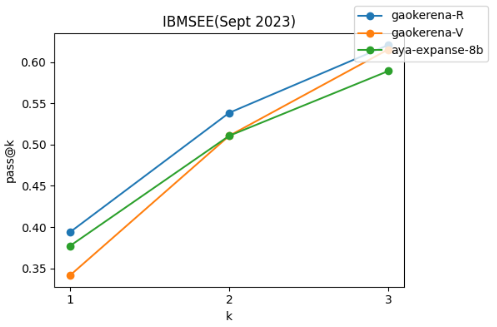
\includegraphics[width=1.0\linewidth]{fig4.png}
    \caption{Pass@k results on the FA\_MED\_MMLU dataset using Chain-of-Thought prompting}
    \label{fig4}
\end{figure}

\begin{figure}[h]
    \centering
    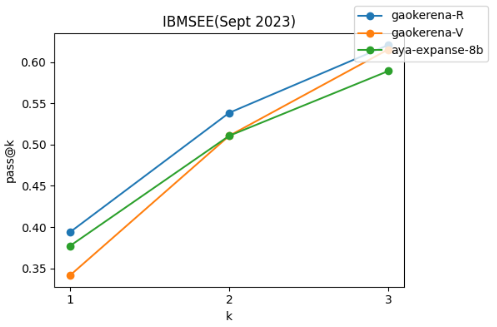
\includegraphics[width=0.8\linewidth]{fig5.png}
    \caption{Pass@k results on the IBMSEE (September 2023) dataset using Chain-of-Thought prompting}
    \label{fig5}
\end{figure}

           \subsection{Medical Knowledge}
As mentioned earlier, gaokerena-V possesses a broader base of medical knowledge compared to the newer gaokerena-R model, primarily because it was trained on a significantly larger and more diverse corpus of medical data.  
This difference becomes evident when both models are evaluated using direct question–answer prompting, rather than being asked to generate explicit chain-of-thought reasoning trajectories.  
As shown in Table
\ref{tab:med_knowledge_comparison}, under this direct prompting setting, gaokerena-V demonstrates superior performance, reflecting its stronger memorization and factual recall abilities derived from large-scale medical pretraining.  
Interestingly, the approximately equal performance of gaokerena-R and its baseline aya-expanse-8b in this same direct prompting setup indicates that gaokerena-R’s superior results in the chain-of-thought setting stem primarily from its enhanced reasoning skills rather than from increased medical knowledge.
 


	\begin{table}[ht]
		\centering
		\caption{Straight Prompted Performance}
		\begin{tabular}{|l|c|c|c|}  
			\hline
			\textbf{} & \textbf{gao} & \textbf{gao} & \textbf{aya-} \\ 
			& \textbf{kerena-R} &  \textbf{kerena-V} & \textbf{expanse-8b} \\
			&   & &(baseline)  \\ \hline
			MMLU- &  &  &  \\ 
			anatomy(fa)  & 41.48 & \textbf{48.14}  & 40.74  \\ \hline
			MMLU- &    &   &   \\
			medical-genetics(fa) & 49.0  & \textbf{53.0}  &  49.0 \\ \hline
			MMLU- &  &    &  \\
			college-medicine(fa) & \textbf{46.24} & 43.93  & 44.51   \\ \hline
			MMLU- &    &  &  \\
			clinical-knowledge(fa) & 52.45 & \textbf{55.47}  & 52.07  \\ \hline
			MMLU- &  &  &  \\
			professional-& 41.91  & \textbf{47.05}  & 45.58   \\
                        medicine(fa)& &   &   \\ \hline
			MMLU- &  &  &  \\
			college-biology(fa)& 44.44 & \textbf{47.22}  &  45.14 \\ \hline
			MMLU(avg) & 46.28 & \textbf{49.31}  & 46.64 \\ \hline
			IBMSEE Sept2023 & 35.11  &\textbf{38.69} & 34.52  \\ \hline
			Number of&  &  &  \\
			parameters & 8b & 8b & 8b \\ \hline
			inference time & $\approx10s$ & $\approx 10s$ & $\approx 10s$ \\  \hline
		\end{tabular}
		\label{tab:med_knowledge_comparison}
	\end{table}


           \subsection{Final Evaluation}
As previously discussed, gaokerena-V performs better when prompted directly, whereas gaokerena-R excels when prompted with a Chain-of-Thought (CoT) format that encourages step-by-step reasoning before producing an answer. One key advantage of CoT prompting—particularly when combined with multiple sampling and majority voting—is that it provides a natural measure of model certainty. If the generated responses converge on the same option across samples, the model can be considered confident; conversely, a wide dispersion among responses indicates uncertainty. This approach offers a practical alternative to directly querying the model’s self-assessed confidence
\cite{b27}
, a capability that smaller models generally lack due to their limited self-awareness and introspective reasoning abilities.

In cases where gaokerena-R exhibits uncertainty (i.e., when multiple distinct answers are produced), we employ the baseline model, aya-expanse-8b, as an auxiliary verifier. The outputs from gaokerena-R are presented to aya-expanse-8b, which is tasked with selecting the option containing the least incorrect or inconsistent information. This hybrid evaluation framework enables us to combine the reasoning strengths of gaokerena-R with the broader knowledge coverage of aya-expanse-8b. 

Accordingly, we compare two configurations, as summarized in Table
\ref{tab:med_opns_comparison}.
 In the first configuration , gaokerena-V is evaluated using direct prompting without any reasoning guidance. In the second configuration , gaokerena-R is prompted with a Chain-of-Thought (CoT) format, and in cases of uncertainty, its generated answers are verified by aya-expanse-8b to identify the most reliable response.

	\begin{table}[ht]
		\centering
		\caption{Evaluation of two different configurations}
		\begin{tabular}{|l|c|c|}  
			\hline
			\textbf{} & \textbf{gaokerena-R} & \textbf{gaokerena-V}  \\ 
			& \textbf{+} &   \\
			& \textbf{ aya-expanse-8b}  &     \\ 
                        & \textbf{(verifier)}  &     \\ \hline
			MMLU- &  &    \\ 
			anatomy(fa)  & 47.40  & \textbf{48.14}   \\ \hline
			MMLU- &   &      \\
			medical-genetics(fa) & \textbf{56.0}  & 53.0   \\ \hline
			MMLU- &  &      \\
			college-medicine(fa) & \textbf{50.28} & 43.93    \\ \hline
			MMLU- &    &    \\
			clinical-knowledge(fa) & \textbf{58.86}  & 55.47  \\ \hline
			MMLU- &  &    \\
			professional-& \textbf{48.89} & 47.05  \\
                        medicine(fa)& &      \\ \hline
			MMLU- &  &   \\
			college-biology(fa)& \textbf{54.86} & 47.22   \\ \hline
			MMLU(avg) & \textbf{52.98}  & 49.31   \\ \hline
			IBMSEE Sept2023 & \textbf{46.42}  &38.69   \\ \hline
                        prompt & COT for the main model & Straight   \\ 
                        &            Straight for the verifier   &   \\ \hline
			inference time & $\approx 5 \times 35 + 8 s$ & $\approx 10s$  \\  \hline
		\end{tabular}
		\label{tab:med_opns_comparison}
	\end{table}
        
\section{Future Research}
The results show that gaokerena-V performs better with direct prompts, while gaokerena-R excels with chain-of-thought (CoT) prompts.  
This indicates that both models are prompt-dependent, as their performance varies with the prompting style.  
Future research should aim to develop prompt-invariant medical language models that integrate strong reasoning skills and medical knowledge, achieving superior performance regardless of the prompt format.  
Achieving prompt invariance would represent an important step toward more reliable and generalizable small Persian medical language models.


	
	
	\begin{thebibliography}{00}
              \bibitem{b1}
              Vaswani, Ashish, et al. "Attention is all you need." Advances in neural information processing systems 30 (2017).
              \bibitem{b2}
              Kahneman, Daniel. "Thinking, fast and slow." Farrar, Straus and Giroux (2011).
              \bibitem{b3}
              Bengio, Yoshua. "From system 1 deep learning to system 2 deep learning." Neural Information Processing Systems. 2019. 
              \bibitem{b4}
              Wei, Jason, et al. "Chain-of-thought prompting elicits reasoning in large language models." Advances in neural information processing systems 35 (2022): 24824-24837.
              \bibitem{b5}
              Lee, Harrison, et al. "Rlaif vs. rlhf: Scaling reinforcement learning from human feedback with ai feedback, 2024." URL https://arxiv. org/abs/2309.00267 2309 (2023).
             \bibitem{b6}
             Rafailov, Rafael, et al. "Direct preference optimization: Your language model is secretly a reward model." Advances in neural information processing systems 36 (2023): 53728-53741.
             \bibitem{b7}
             Ghassabi, Mehrdad, et al. "Leveraging Online Data to Enhance Medical Knowledge in a Small Persian Language Model." arXiv preprint arXiv:2505.16000 (2025).
             \bibitem{b8}
             Dang, John, et al. "Aya expanse: Combining research breakthroughs for a new multilingual frontier." arXiv preprint arXiv:2412.04261 (2024).
             \bibitem{b9}
             Pan, Liangming, et al. "Automatically correcting large language models: Surveying the landscape of diverse self-correction strategies." arXiv preprint arXiv:2308.03188 (2023).
             \bibitem{b10}
             Jiang, Shuyang, et al. "MedS$^ 3$: Towards Medical Slow Thinking with Self-Evolved Soft Dual-sided Process Supervision." arXiv preprint arXiv:2501.12051 (2025).
             \bibitem{b11}
             Coulom, Rémi. "Efficient selectivity and backup operators in Monte-Carlo tree search." International conference on computers and games. Berlin, Heidelberg: Springer Berlin Heidelberg, 2006.
             \bibitem{b12}
             Rafailov, Rafael, et al. "Direct preference optimization: Your language model is secretly a reward model." Advances in neural information processing systems 36 (2023): 53728-53741.
             \bibitem{b13}
             Wu, Juncheng, et al. "Medreason: Eliciting factual medical reasoning steps in llms via knowledge graphs. ArXiv, abs/2504.00993, 2025."
             \bibitem{b14}
             Chen, Junying, et al. "Huatuogpt-o1, towards medical complex reasoning with llms." arXiv preprint arXiv:2412.18925 (2024).
             \bibitem{b15}
             Guo, Daya, et al. "Deepseek-r1: Incentivizing reasoning capability in llms via reinforcement learning." arXiv preprint arXiv:2501.12948 (2025).
             \bibitem{b16}
             Shao, Zhihong, et al. "Deepseekmath: Pushing the limits of mathematical reasoning in open language models." arXiv preprint arXiv:2402.03300 (2024).
             \bibitem{b17}
             Wu, Tianhao, et al. "Thinking llms: General instruction following with thought generation." arXiv preprint arXiv:2410.10630 (2024).
             \bibitem{b18}
             Ho, Namgyu, Laura Schmid, and Se-Young Yun. "Large language models are reasoning teachers." arXiv preprint arXiv:2212.10071 (2022).
             \bibitem{b19}
             Bi, Xiao, et al. "Deepseek llm: Scaling open-source language models with longtermism." arXiv preprint arXiv:2401.02954 (2024).
             \bibitem{b20}
             Pal, Ankit, Logesh Kumar Umapathi, and Malaikannan Sankarasubbu. "Medmcqa: A large-scale multi-subject multi-choice dataset for medical domain question answering." Conference on health, inference, and learning. PMLR, 2022.
             \bibitem{b21}
             xAI. "Grok 3 Beta — The Age of Reasoning Agents." xAI Blog, 17 Feb. 2025, x.ai/news/grok-3.
             \bibitem{b22}
             Achiam, Josh, et al. "Gpt-4 technical report." arXiv preprint arXiv:2303.08774 (2023).
             \bibitem{b23}
             Ranjbar Kalahroodi, Mohammad Javad, et al. "PersianMedQA: Evaluating Large Language Models on a Persian-English Bilingual Medical Question Answering Benchmark." arXiv preprint arXiv:2506.00250 (2025).
             \bibitem{b24}
             Canadian Climate Institute. “The Big Switch in Canada’s Electricity Emissions.” 440 Megatonnes, 2023, https://440megatonnes.ca/insight/the-big-switch-in-canada-s-electricity-emissions
. Accessed 21 Oct. 2025.
             \bibitem{b25}
             Lacoste, Alexandre, et al. "Quantifying the carbon emissions of machine learning." arXiv preprint arXiv:1910.09700 (2019).
             \bibitem{b26}
             Brown, Bradley, et al. "Large language monkeys: Scaling inference compute with repeated sampling." arXiv preprint arXiv:2407.21787 (2024).
             \bibitem{b27}
             Zhang, Mozhi, et al. "Calibrating the confidence of large language models by eliciting fidelity." arXiv preprint arXiv:2404.02655 (2024).
            
         
	\end{thebibliography}
	
	
\end{document}